\documentclass[11pt, a4paper]{article}
\usepackage[utf8]{inputenc}
\usepackage{minted}
\usepackage{hyperref}
\usepackage{graphicx}
\usepackage{subcaption}
\graphicspath{{./images/}}

\setlength{\parindent}{0em}
\setlength{\parskip}{1em}

\begin{document}
\title{Concurrency}
\author{Samuel Navarro}
\date{\today}
\maketitle
\tableofcontents{}

\section{Introduction}%
\label{sec:introduction}

Concurrency means that a single system is performing multiple, independent tasks in parallel rather than sequentially as before. Such a system is called a multi-tasking system. 

Multi-tasking does not require multiple processes or multiple cores. Dividing a program execution into many small bits and pieces and by interleaving them with a bits of pieces of other programs we create the illusion of parallelism, which is maintained by the OS. Under the hood we have an extremely fast switching of tasks. 

But true concurrency with tasks that are running at the same time require a parallel architecture. This might mean having multiple processors or multiple cores, or maybe both multiple cores within a processor. This is called \textbf{hardware concurrency.}


An important measure which helps to gauge how many independent tasks can be run in parallel, this is the number of hardware threads on a system. 


\section{Introduction and Running Threads}%
\label{sec:introduction_and_running_threads}



\subsection{Processes and Threads}%
\label{sec:processes_and_threads}



A parallel path of execution is one which runs concurrently with the main program and is thus asynchronous. In contrast to synchronous programs, the main program can continue with its line of execution without the need to wait for the parallel task to complete. The following figure illustrates this difference.




\begin{figure}[htpb!]
	\centering
	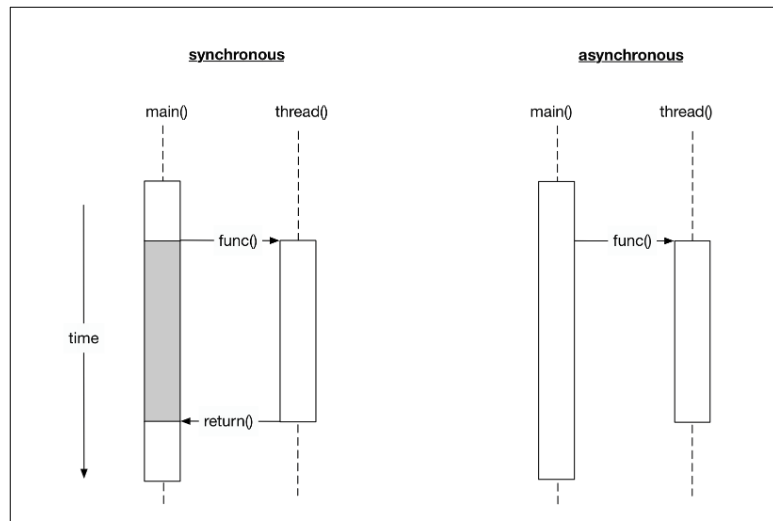
\includegraphics[width=0.8\linewidth]{async_sync}
	\caption{Asynchronous vs Synchronous}
	\label{fig:async_sync}
\end{figure}


A \textbf{process} (also called a \textbf{task}) is a computer program at runtime. It is comprised of the runtime environment provided by the OS, as well as of the embedded binary code of the program during execution. A \textbf{process} is controlled by the OS through certain actions with which it sets the process into one of several carefully defined states:



\begin{figure}[htpb!]
	\centering
	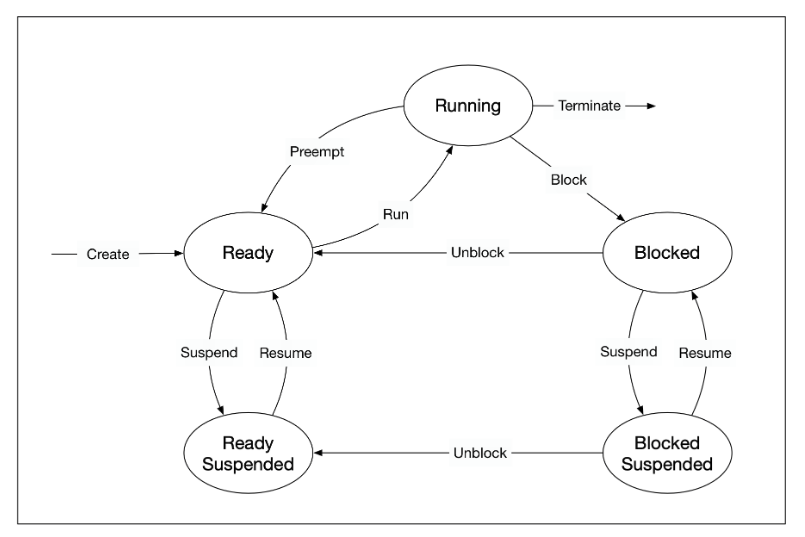
\includegraphics[width=0.8\linewidth]{process}
	\caption{Process}
	\label{fig:process}
\end{figure}


\begin{itemize}
	\item \textbf{Ready} : After its creation, a process enters the ready state and is loaded into main memory. The process now is ready to run and is waiting for CPU time to be executed. Processes that are ready for execution by the CPU are stored in a queue managed by the OS.
	\item \textbf{Running} : The operating system has selected the process for execution and the instructions within the process are executed on one or more of the available CPU cores.
	\item \textbf{Blocked} : A process that is blocked is one that is waiting for an event (such as a system resource becoming available) or the completion of an I/O operation.
	\item \textbf{Terminated} : When a process completes its execution or when it is being explicitly killed, it changes to the "terminated" state. The underlying program is no longer executing, but the process remains in the process table as a "zombie process". When it is finally removed from the process table, its lifetime ends.
	\item \textbf{Ready suspended}: A process that was initially in ready state but has been swapped out of main memory and placed onto external storage is said to be in suspend ready state. The process will transition back to ready state whenever it is moved to main memory again.
	\item \textbf{Blocked suspended} : A process that is blocked may also be swapped out of main memory. It may be swapped back in again under the same conditions as a "ready suspended" process. In such a case, the process will move to the blocked state, and may still be waiting for a resource to become available.
\end{itemize}





Processes are managed by the scheduler of the OS. The scheduler can either let a process run until it ends or blocks (non-interrupting scheduler), or it can ensure that the currently running process is interrupted after a short period of time. The scheduler can switch back and forth between different active processes (interrupting scheduler), alternately assigning them CPU time. The latter is the typical scheduling strategy of any modern operating system.

Since the administration of processes is computationally taxing, operating systems support a more resource-friendly way of realizing concurrent operations: the threads.


A \textit{thread} represents a concurrent execution unit within a process. In contrast to full-blown processes as described above, threads are characterized as light-weight processes (LWP). There are significantly easier to create and destroy: In many systems the creation of a thread is up to 100 times faster than the creation of a process. This is especially advantageous in situations, when the need for concurrent operations changes dynamically. 


\begin{figure}[htpb!]
	\centering
	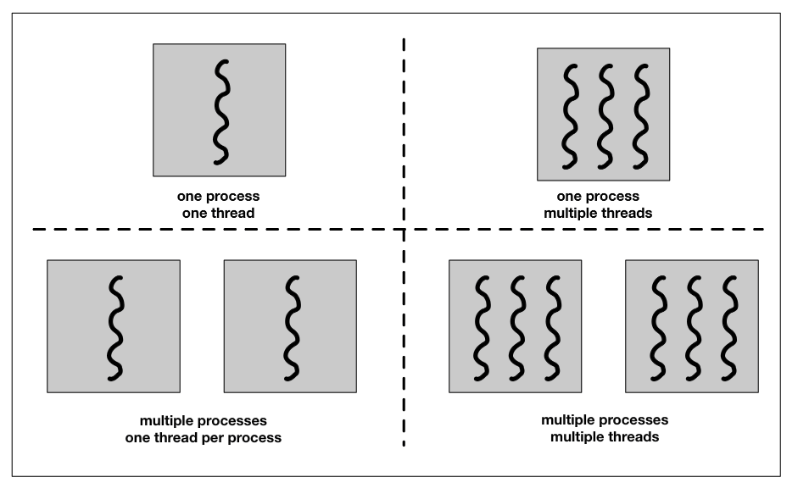
\includegraphics[width=0.8\linewidth]{process_threads}
	\caption{Process and Threads}
	\label{fig:process_threads}
\end{figure}




Threads exist within processes and share their resources. As illustrated by the Figure~\ref{fig:process_threads}, a process can contain several threads or - if no parallel processing is provided for in the program flow - only a single thread.

A major difference between a process and a thread is that each process has its own address space, while a thread does not require a new address space to be created. All the threads in a process can access its shared memory. Threads also share other OS dependent resources such as processors, files, and network connections. As a result, the management overhead for threads is typically less than for processes. Threads, however, are not protected against each other and must carefully synchronize when accessing the shared process resources to avoid conflicts.


Similar to processes, threads exist in different states, which are illustrated in the Figure~\ref{fig:threads}: 


\begin{figure}[htpb!]
	\centering
	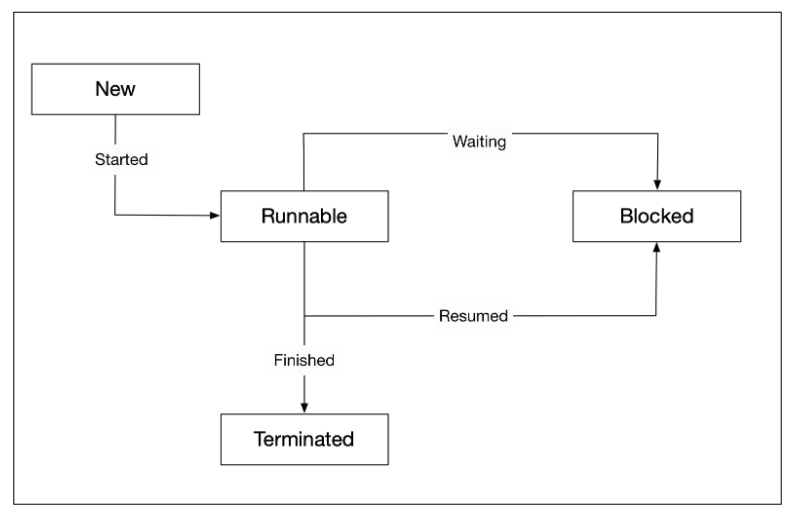
\includegraphics[width=0.8\linewidth]{threads}
	\caption{Threads}
	\label{fig:threads}
\end{figure}


\begin{itemize}
	\item \textbf{New} : A thread is in this state once it has been created. Until it is actually running, it will not take any CPU resources.
	\item \textbf{Runnable} : In this state, a thread might actually be running or it might be ready to run at any instant of time. It is the responsibility of the thread scheduler to assign CPU time to the thread.
	\item \textbf{Blocked} : A thread might be in this state, when it is waiting for I/O operations to complete. When blocked, a thread cannot continue its execution any further until it is moved to the runnable state again. It will not consume any CPU time in this state. The thread scheduler is responsible for reactivating the thread.
\end{itemize}




\begin{itemize}
	\item In a concurrent program, \textbf{threads} share memory. Thus, many \textbf{threads} can access and modify the same memory.
	\item Creating a \textbf{process} is fairly resource-intensive. It is generally more efficient to use several \textbf{threads} within a \textbf{process}.
	\item In contrast to a \textbf{process}, \textbf{threads} are characterized as light-weight. They are significantly easier to create and destroy.
	\item Inter-thread communication can be faster than inter-process communication.
\end{itemize}


\subsection{Starting a Second Thread}%
\label{sec:starting_a_second_thread}



If we want to start a second thread in addition to the main thread of our program, we need to construct a thread object and pass it the function we want to be executed by the thread. Once the thread enters the runnable state, the execution of the associated thread function may start at any point in time.

\texttt{std::thread t (threadFunction);} 


After the thread object has been constructed, the main thread will continue and execute the remaining instructions until it reaches the end and returns. It is possible that by this point in time, the thread will also have finished. But if this is not the case, the main program will terminate and the resources of the associated process will be freed by the OS. As the thread exists within the process, it can no longer access those resources and thus not finish its execution as intended.

To prevent this from happening and have the main program wait for the thread to finish the execution of the thread function, we need to call \texttt{join()} on the thread object. This call will only return when the thread reaches the end of the thread function and block the main thread until then.  

An example of this is in the file \texttt{main\_and\_sec\_threads.cpp}


\subsubsection{Randomness of events}%
\label{sub:randomness_of_events}

One very important trait of concurrent programs is their non-deterministic behavior. It can not be predicted which thread the scheduler will execute at which point in time. In the code on \texttt{randomness\_of\_events.cpp}, the amount of work to be performed both in the thread function and in main has been split into two separate jobs. The output in the console differs. 


\textbf{We can use \texttt{join()} as a barrier}

Because the order of execution is determined by the scheduler, if we wanted to ensure that the thread function completed its work before the main function started its own work \textbf{(because it might be waiting for a result to be available)}, we could achieve this by repositioning the call to join.


In the file, the \texttt{.join()} can be moved to before the work in \texttt{main()}. The order of execution now always looks the same.


\subsubsection{Detach}%
\label{sub:detach}



Let us now take a look at what happens if we don’t join a thread before its destructor is called. When we comment out join in the example above and then run the program again, it aborts with an error. The reason why this is done is that the designers of the C++ standard wanted to make debugging a multi-threaded program easier: Having the program crash forces the programmer to remember joining the threads that are created in a proper way. Such a hard error is usually much easier to detect than soft errors that do not show themselves so obviously.

There are some situations however, where it might make sense to not wait for a thread to finish its work. This can be achieved by "detaching" the thread, by which the internal state variable "joinable" is set to "false". This works by calling the \texttt{detach()} method on the thread. \textbf{The destructor of a detached thread does nothing: It neither blocks nor does it terminate the thread}. In the following example, detach is called on the thread object, which causes the main thread to immediately continue until it reaches the end of the program code and returns. Note that a detached thread can not be joined ever again.


Programmers should be very careful though when using the \texttt{detach()} method. You have to make sure that the thread does not access any data that might get out of scope or be deleted. Also, we do not want our program to terminate with threads still running. Should this happen, such threads will be terminated very harshly without giving them the chance to properly clean up their resources - what would usually happen in the destructor. So a well-designed program usually has a well-designed mechanism for joining all threads before exiting.





\subsection{Starting a Thread with a Function Object}%
\label{sec:starting_a_thread_with_a_function_object}

We now want to pass a function object instance to the thread. This is basically an instance of a class that implements the function call operator. This can be very useful to passing data through threads. Another way to pass data and also start a thread with a very small code footprint is to use a so-called Lambda function. 



Passing functions to other functions is one form of a \textit{callable object}.

In C++, callable objects are objects that can appear as the left-hand operand of the call operator. These can be pointers to functions, objects of a class that defines an overloaded function call operator and \textit{lambdas}, with which function objects can be created in a very simple way. In the context of \textbf{concurrency}, we can use callable objects to attach a function to a thread. 

In the Section~\ref{sec:starting_a_second_thread} we constructed a thread object by passing a function to it without any arguments. If we were limited to this approach, the only way to make data available from within the thread function would be to use global variables - \textit{which is definitely not recommendable and also incredibly messy.}





The extra parenthesis in the file \texttt{mostVexingParse} is known as C++'s \textit{most vexing parse}, which is a specific form of syntactic ambiguity resolution in the C++ programming language.

The \textit{"most vexing parse"} comes from a rule in C++ that says that anything that could be considered as a function declaration, the compiler should parse it as a function declaration - even if it could be interpreted as something else.


The line:

\texttt{std::thread t(Vehicle());} 

is seemingly ambiguous, since it could be interpreted either as:

\begin{enumerate}
	\item a variable definition for variable t of class \texttt{std::thread}, initialized with an anonymous instance of class Vehicle, or
	\item a function declaration for a function t that return an object of type \texttt{std::thread}  and has a single (unnamed) parameter that is a pointer to function returning an object of type Vehicle.
\end{enumerate}


Most programmers would presumable expect the first case to be true, but the C++ standard requires it to be interpreted as the second - hence the compiler warning. 


There are three ways of forcing the compiler to consider the line as the first case, which would create the thread object we want:


\begin{itemize}
  \item Add an extra pair of parentheses: \texttt{std::thread t1 ( (Vehicle()) );} 
	\item Use copy initialization. \texttt{std::thread t2 = std::thread( Vehicle() ) ;} 
	\item Use uniform initialization with braces. \texttt{std::thread t3\{Vehicle()\};} 
\end{itemize}

Whichever option we use, the idea is the same: the function object is copied into internal storage accessible to the new thread, and the new thread invokes the operator \texttt{()}. Th \texttt{Vehicle()} class can of course have data members and other member functions too, and this is one way of passing data to the thread function: pass it in as a constructor argument and store it as a data member.

File: \texttt{PassingDataToThread.cpp} 




\subsubsection{Lambdas}%
\label{sub:lambdas}


Another useful way of starting a thread and passing information to it is by using a lambda expression. C++ Lambdas have the properties of being unnamed and capturing variables from the surrounding context, but lack the ability to execute and return functions. 

A Lambda is often used as an argument for functions that can take a callable object. A Lambda is a function object, so it has a type and can be stored and passed around. Its result object is called a \textit{"closure"}, which can be called using the operator \texttt{()} 

It formally consists of three parts: a capture list \texttt{[]}, a parameter list \texttt{()} and a main part \texttt{\{\}}, which contains the code to be executed when the lambda is called. Note that in principal all parts could be empty.

The capture list \texttt{[]}: By default, variables outside of the enclosing {} around the main part of the Lambda can not be accessed. By adding a variable to the capture list however, it becomes available within the Lambda \textbf{either as a copy or as a reference}. The captured variables become a part of the Lambda.

By default, variables in the capture block can not be modified within the Lambda. Using the keyword "mutable" allows to modify the parameters captured by copy, and to call their non-const member functions within the body of the Lambda.


Even though we have been using Lambdas in the above example in various ways, it is important to note that a Lambda does not exist at runtime. The runtime effect of a Lambda is the generation of an object, which is known as closure. The difference between a Lambda and the corresponding closure is similar to the distinction between a class and an instance of the class. A class exists only in the source code while the objects created from it exist at runtime.

We can use (a copy of) the closure (i.e. f0, f1, …) to execute the code within the Lambda at a position in our program different to the line where the function object was created.

The parameter list () : The way parameters are passed to a Lambda is basically identical to calling a regular function. If the Lambda takes no arguments, these parentheses can be omitted (except when "mutable" is used).



\textbf{Question} What's the difference between capture list and parameter list. See this \href{https://stackoverflow.com/questions/28669941/c-lambdas-capture-list-vs-parameter-list}{link}

It seems that the capture list is to keep a state.


\begin{listing}
\begin{minted}[linenos,numbersep=5pt,frame=lines,framesep=2mm]{cpp}
#include <iostream>

int main(){
	const auto addSome = [](double some){
		return [some](double val){ return some + val;};
	};


	const auto addFive = addSome(5);

	std::cout << addFive(2) << std::endl;
	std::cout << addFive(3) << std::endl;
	/*
  OUTPUT:
  7
	8
	* */
	return 0;
}
\end{minted}
\caption{Capture vs Parameter List in Lambda Functions}
\label{lst:capture_vs_parameter_list_in_lambda_functions}
\end{listing}









Let's say we have this code snippet:




\begin{listing}
\begin{minted}[linenos,numbersep=5pt,frame=lines,framesep=2mm]{cpp}
#include <iostream>

int main()
{
    int id = 0; // Define an integer variable

    // capture by reference (immutable)
    auto f0 = [&id]() { std::cout << "a) ID in Lambda = " << id << std::endl; };

    // capture by value (mutable)
    auto f1 = [id]() mutable { std::cout << "b) ID in Lambda = " << ++id << std::endl; };
    f1(); // call the closure and execute the code witin the Lambda
    std::cout << "c) ID in Main = " << id << std::endl;

    // capture by reference (mutable)
    auto f2 = [&id]() mutable { std::cout << "d) ID in Lambda = " << ++id << std::endl; };
    f2(); 
    std::cout << "e) ID in Main = " << id << std::endl; 

    // pass parameter 
    auto f3 = [](const int id) { std::cout << "f) ID in Lambda = " << id << std::endl; };   
		//Before we pass id into it, we increase it by one.
		//That's why we have id = 2
    f3(++id);

    // observe the effect of capturing by reference at an earlier point in time
		// Because we pass by reference the id, we have Id=2
    f0(); 

    return 0;
}
\end{minted}
\caption{Capture Variables by Value and Reference}
\label{lst:capture_variables_by_value_and_reference}
\end{listing}


Pass by value means that we are going to make a copy of the parameter; we're not going to change the original ID. But, because the lambda is \texttt{mutable} that means that ID can be change within the Lambda itself. 


In Listing~\ref{lst:capture_variables_by_value_and_reference}. The output will be:
\begin{itemize}
	\item b) ID lambda = 1
	\item c) ID Main = 0
	\item d) ID lambda = 1
	\item e) ID Main = 1
	\item f) ID lambda = 2
	\item a) Id lambda = 2
\end{itemize}





Another example is in file: \texttt{startThreadsLambdas.cpp}. Here, the output in the main thread is generated first, at which point the variable ID has taken the value 1. Then, the call-by-value thread is executed with ID at a value of 0. Then, the call-by-reference thread is executed with ID at a value of 1. This illustrates the effect of passing a value by reference : when the data to which the reference refers changes before the thread is executed, those changes will be visible to the thread. We will see other examples of such behavior later in the course, as this is a primary source of concurrency bugs.


Intuition: The lambda which passes by value the id, gets id = 0. Also, the pass by reference function gets id=0, but, by the time the function finishes its work, id now has turned into 1.






\subsection{Starting a Thread with Variadic Templates and Member Functions}%
\label{sec:starting_a_thread_with_variadic_templates_and_member_functions}


\textbf{Variadic Templates}: They allow the definition of functions that take a varying number of arguments which is handy in concurrency because we can use them to pass several arguments to a thread. 

\textbf{Como nota importante:} con Variadic Templates se pasan los argumentos en el mismo orden.

\textbf{Member Functions} We can pass arguments to a thread by reference, but what if we wish to run a function other than the function call operator. We want to run functions of already existent objects. 



We have seen that one way to pass arguments in to the thread function is to package them in a class using the function call operator. Even though this worked well, it would be very cumbersome to write a special class every time we need to pass data to a thread. We can also use a Lambda that captures the arguments and then calls the function. But there is a simpler way: The thread constructor may be called with a function and all its arguments. That is possible because the thread constructor is a \textit{variadic template} that takes multiple arguments.


\subsubsection{Variadic Templates}%
\label{sub:variadic_templates}



The need for \textbf{variadic templates} could be illustrated in the Listing~\ref{lst:variadic_templates}. The second thread object is constructed with a function \texttt{printIDAndName}, which requires an int and a string, but if we only pass a single argument to the thread when calling\texttt{printIDAndName} a compiler error will occur.  



\begin{listing}
\begin{minted}[linenos,numbersep=5pt,frame=lines,framesep=2mm]{cpp}
#include <iostream>
#include <thread>
#include <string>

void printID(int id)
{
    std::this_thread::sleep_for(std::chrono::milliseconds(50));
    std::cout << "ID = " << id << std::endl;
    
}

void printIDAndName(int id, std::string name)
{
    std::this_thread::sleep_for(std::chrono::milliseconds(100));
    std::cout << "ID = " << id << ", name = " << name << std::endl;
}

int main()
{
    int id = 0; // Define an integer variable

    // starting threads using variadic templates
    std::thread t1(printID, id);
    std::thread t2(printIDAndName, ++id, "MyString");
    std::thread t3(printIDAndName, ++id); // this procudes a compiler error

    // wait for threads before returning
    t1.join();
    t2.join();
    //t3.join();


    return 0;
}
\end{minted}
\caption{Variadic Templates}
\label{lst:variadic_templates}
\end{listing}




There is one more difference between calling a function directly and passing it to a thread: With the former, arguments may be passed by value, by reference or by using move semantics - depending on the signature of the function. When calling a function using a variadic template, the arguments are by default either moved or copied - depending on wether they are rvalues or lvalues. There are ways however which allow us to overwrite this behavior. If you want to move an lvalue for example, we can call std::move. 


In the file \texttt{MoveVsCopybyValue.cpp}, two threads are started. One where the string is \textbf{copied by value}. This allows us to print name1 even after \texttt{join} has been called. The second one is passed to the thread function using \textbf{move semantics}, which means that it is not available any more after \texttt{join} has been called.


In the file \texttt{PassDataAsRef.cpp}, when passing the string variable name to the thread funciton, we need to explicity mark it as a reference, so the compiler threat it as such. This is done using \texttt{std::ref}.


Even though the code works, we are now sharing mutable data between threads - \textbf{which is a primary source for concurrency bugs.}

\subsubsection{Starting Threads with Member Functions}%
\label{sub:starting_threads_with_member_functions}



What if we want to run a member function other than the function call operator, such as a member function of an existing object?. In C++, for calling member functions, the \texttt{std::thread} function requires an additional argument for the object on which to invoke the member function.


In the \texttt{ThreadsMemberFunc.cpp}, the Vehicle object v1 is passed to the thread function by value, thus a copy is made which does not affect the \textit{original} living in the main thread. That's why changes to its members variable \texttt{\_id} will thus not show when printing later in main. 

In the second Vehicle object, because it's passed by reference, changes to its \texttt{\_id} variable will also be visible in the main thread. 


Another thing to consider is that we have to ensure that the existence of \texttt{v2} outlives the completion of the thread \texttt{t2} - otherwise there will be an attempt to access an invalidated memory address. An alternative is to use a heap-allocated object and a reference-counted pointer such as \texttt{std::shared\_ptr<Vehicle>} to ensure that the object lives as long as it takes the thread to finish its work. The file 




\subsection{Running Multiple Threads}%
\label{sec:running_multiple_threads}


\subsubsection{Fork-Join Parallelism}%
\label{sub:fork_join_parallelism}

The basic mechanism of this concept follows a simple three-step pattern:

\begin{enumerate}
	\item Split the flow of execution into a parallel thread ( \textit{"fork"})
	\item Perform some work in both the main thread and the parallel thread.
	\item Wait for the parallel thread to finish and unite the split flow of execution again \textit{("join")}.
\end{enumerate}





\begin{figure}[htpb!]
	\centering
	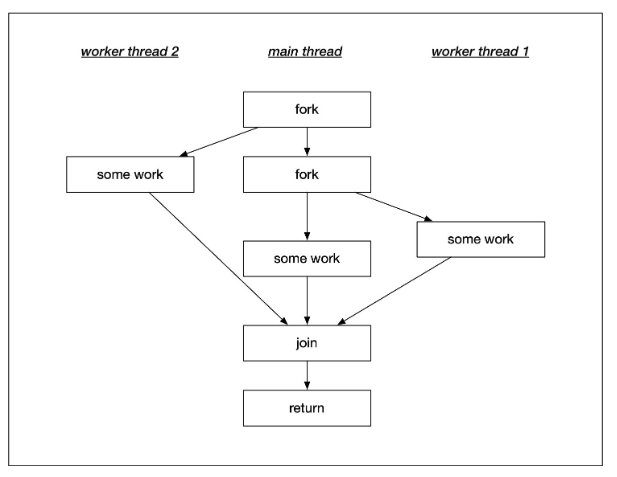
\includegraphics[width=0.8\linewidth]{fork_join}
	\caption{Fork-Join Parallelism}
	\label{fig:fork_join_parallelism}
\end{figure}

In the main thread, the program flow is forked into three parallel branches. In both worker branches, some work is performed - which is why threads are often referred to as \textit{"worker threads"}. Once the work is completed, the flow of execution is united again in the main function using the \texttt{join()}  command. In this example, join acts as a barrier where all threads are united. The execution of main is in fact halted, until both worker threads have successfully completed their respective work. 



In the \texttt{forkJoinParallelism.cpp} file, if we try to compile the program using the \texttt{push\_back()} function, we get a compiler error. The problem with our code is that by pushing the thread object into the vector, we attempt to make a copy of it. However, thread objects do not have a copy constructor and thus can not be duplicated. If this were possible, we would create yet another branch in the flow of execution - which is not what we want. The solution to this problem is to use move semantics, which provide a convenient way for the contents of objects to be 'moved' between objects, rather than copied. It might be a good idea at this point to refresh your knowledge on move semantics, on rvalues and lvalues as well as on rvalue references, as we will make use of these concepts throughout the course.

To solve our problem, we can use the function \texttt{emplace\_back()} instead of \texttt{push\_back()} which internally uses move semantics to move our thread object into the vector without making a copy. 

The console output is really messy. the components are completely intermingled. Also, when the program is run several times, the output will look different with each execution.


\begin{itemize}
	\item The order in which threads are executed is non-deterministic. Every time a program is executed, there is a chance for a completely different order of execution.
	\item Threads may get preempted in the middle of execution and another thread may be selected to run.
\end{itemize}


\textbf{These two properties pose a major problem with concurrent applications: A program may run correctly for thousands of times and suddenly, due to a particular interleaving of threads, there might be a problem. From a debugging perspective, such errors are very hard to detect as they can not be reproduced easily.}




In the file \textbf{properMultipleThreads.cpp}: the bug comes from accessing a shared memory location. (Remember that the lambda function in the code used \texttt{id}  by reference.)







\section{Passing Data Between Treads}%
\label{sec:passing_data_between_treads}


\begin{enumerate}
	\item We are going to look at the private communication channel, between two threads that can be used only a single time but at an arbitrary moment in time of our choosing. The concept behind this is called \textbf{promises and futures} and this can be used to pass data as well as exceptions from a worker thread to the parent thread which created the worker.   
	\item We are going to look at the differences between \textbf{threads} and \textbf{tasks.} \textbf{Tasks} are a high level concept where the system can choose whether to execute some code in parallel or synchronously. Also, they make easy to establish a promise future link in our code. This is much less code to write than standard \textbf{threads} we have usen so far. 
	\item Look at the runtime advantage or disadvantage of parallel execution.
	\item Passing data to a thread by value (making a copy of it) as well as using \textbf{move semantics.} Move semantics which avoids making unnecessary copies of your data, while at the same time avoiding some of the dangers of passing by reference. (which has an impact of the variables at main). 
	\item Look at data races which are one of the primary sources of error on concurrent programming. 
\end{enumerate}


\subsection{Promises and Futures}%
\label{sub:promises_and_futures}

Previously, we have look in the ways we can pass data from the parent thread to the worker thread. Now we want to move data from the worker to the parent thread (in this case, the main function). The sending of the channel is \textbf{promise} and the receiving is called \textbf{future} 


We can create a thread that takes a function and we will pass it the promise as an argument as well as the message to be modified. \textbf{Promises} cannot be copied, because the \textbf{promise-future} concept is a two-point communication channel for one-time use. Therefore, we must pass the promise to the thread function using the \texttt{std::move}. 

The thread function takes the promise as an rvalue reference in accordance with move semantics \textbf{(? qué significa esto¿)}. After waiting for several seconds, the message is modified and the method \texttt{set\_value()} is called on the promise. 


Back in the main thread, after starting the thread, the original message is printed to the console. Then, we start listening on the other end of the communication channel by calling the function \texttt{get()} on the future. This method will block until data is available - which happens as soon as \texttt{set\_value} has been called on the promise (from the thread). If the result is movable (which is the case for \texttt{ std::string}), it will be moved - otherwise it will be copied instead. After the data has been received (with a considerable delay), the modified message is printed to the console.


It's also possible that the worker value calls \texttt{set\_vale()} on the promise before \texttt{get()} is called on the future. In this case, \texttt{get()} return immediately without any delay. After \texttt{get()} has been called once, the future is no longer usable. This makes sense as the normal mode of data exchange between \textbf{promise} and \textbf{future} works with \texttt{std::move} - and in this case, the data is no longer available in the channel after the first call to \texttt{get()}. If \texttt{get()} is called a second time, an exception is thrown.



\subsubsection{Get vs Wait}%
\label{ssub:get_vs_wait}


There are some situations where it might be interesting to separate the waiting for the content from the actual retrieving. Futures allow us to do that using the \texttt{wait()} function. This method will block until the future is ready. Once it returns, it is guaranteed that data is available and we can use \texttt{get()} to retrieve it without delay.



In addition to wait, the C++ standard also offers the method \texttt{wait\_for}, which takes a time duration as an input and also waits for a result to become available. The method \texttt{wait\_for()} will block either until the specified timeout duration has elapsed or the result becomes available - whichever comes first. The return value identifies the state of the result.



\subsubsection{Passing Exceptions}%
\label{ssub:passing_exceptions}


The future-promise communication channel may also be used for passing exceptions. This is in the file \texttt{passingExceptions.cpp}.

In the thread function, we need to implement a try-catch block which can be set to catch a particular exception or - as in our case - to catch all exceptions. Instead of setting a value, we now want to throw a \texttt{std::exception} along with a customized error message. In the catch-block, we catch this exception and throw it to the parent thread using the promise with \texttt{set\_exception}. The function \texttt{std::current\_exception} allows us to easily retrieve the exception which has been thrown.

On the parent side, we now need to catch this exception. In order to do this, we can use a try-block around the call to get(). We can set the catch-block to catch all exceptions or - as in this example - we could also catch a particular one such as the standard exception. Calling the method what() on the exception allows us to retrieve the message from the exception - which is the one defined on the promise side of the communication channel.

\textbf{When we run the program, we can see that the exception is being thrown in the worker thread with the main thread printing the corresponding error message to the console.}

So a promise future pair can be used to pass either values or exceptions between threads.


One of the nice thing of using futures is that you can determine the point in time when you want to retrieve data by calling the \texttt{get()}  function. That can be very useful especially when you want to ensure that the result is only available at a certain point in time. Now, there are two major drawbacks from promises and futures.

\begin{enumerate}
	\item Information can only be passed into one direction. (from worker to parent).
	\item They are made for one-time use only. 
\end{enumerate}



\subsection{Threads vs Tasks}%
\label{sub:threads_vs_tasks}


If you want to quickly return data or an exception from worker to parent, a much simpler way than doing it with futures and promises is using \textbf{standard async} instead of standard thread. Calling \textbf{async} generates something called a \textbf{task} which is a high level construct where the system can decide whether to run it in parallel or  asynchronously.  



In the file \texttt{threadsWithAsync.cpp} we are going to change to code so we use \texttt{st::async}  instead of \texttt{std::thread}. 

The first change we are making is in the thread function: We are removing the promise from the argument list as well as the try-catch block. Also, the return type of the function is changed from void to double as the result of the computation will be channeled back to the main thread using a simple return. After these changes, the function has no knowledge of threads, nor of futures or promises - it is a simple function that takes two doubles as arguments and returns a double as a result. Also, it will throw an exception when a division by zero is attempted.

In the main thread, we replace \texttt{std::thread} with \texttt{std::async}. Note that async returns a future, which we will use later in the code to retrieve the value that is returned by the function. A promise, as with \texttt{std::thread}, is no longer needed, so the code becomes much shorter. In the try-catch block, nothing has changed - we are still calling \texttt{get()} on the future in the try-block and exception-handling happens unaltered in the catch-block. Also, we do not need to call \texttt{join()} any more. With async, the thread destructor will be called automatically - which reduces the risk of a concurrency bug.

When we run with \texttt{async}, as expected, the ids between the two threads (main and function) differ from each other - they are running in parallel. However, one of the major differences between \texttt{std::thread} and \texttt{std::async} is that with the latter, the system decides whether the associate function should be run asynchronously or synchronously. We can directly influence on this by adjusting the launch parameters of \texttt{std::async}. 

This is reflected in the line \texttt{std::future<double> ftr = std::async(std::launch::deferred, ...)} of the file \texttt{asyncForceParallel.cpp }


If we were to use the launch option \textit{"async"} instead of \textit{"deferred"} we would enforce an asynchronous execution whereas the option \textit{"any"} would leave it to the system to decide (which is the default).

At this point, let us compare std::thread with std::async: Internally, std::async creates a promise, gets a future from it and runs a template function that takes the promise, calls our function and then either sets the value or the exception of that promise - depending on function behavior. The code used internally by std::async is more or less identical to the code we used in the previous example (\texttt{passinExceptions.cpp} in the PromisesAndFutures folder)  , except that this time it has been generated by the compiler and it is hidden from us - which means that the code we write appears much cleaner and leaner. Also, std::async makes it possible to control the amount of concurrency by passing an optional launch parameter, which enforces either synchronous or asynchronous behavior. This ability, especially when left to the system, allows us to prevent an overload of threads, which would eventually slow down the system as threads consume resources for both management and communication. If we were to use too many threads, the increased resource consumption would outweigh the advantages of parallelism and slow down the program. By leaving the decision to the system, we can ensure that the number of threads is chosen in a carefully balanced way that optimizes runtime performance by looking at the current workload of the system and the multi-core architecture of the system.



\subsubsection{Task-based Concurrency}%
\label{ssub:task_based_concurrency}

Determining the optimal number of threads to use is a hard problem. It usually depends on the number of available cores whether it makes sense to execute code as a thread or in a sequential manner. The use of \texttt{std::async} (and thus tasks) take the burden of this decision away from the user and let the system decide whether to execute the code sequentially or as a thread. With tasks, the programmer decides what \textbf{CAN} be run in parallel in principle and the system then decides at runtime what \textbf{WILL} be run in parallel.

Internally, this is achieved by using thread-pools which represent the number of available threads based on the cores/processors as well as by using work-stealing queues, where tasks are re-distributed among the available processors dynamically.


We can see the idea of \textbf{work-stealing queue} in the Figure~\ref{fig:work_stealing_queues}. The first core in the example is heavily oversubscribed with several tasks that are waiting to be executed. he idea of a work-stealing queue is to have a watchdog program running in the background that regularly monitors the amount of work performed by each processor and redistributes it as needed. So, in our example, the tasks waiting would be shifted (or \textit{"stolen"}) from busy cores and added to available free cores.

A work distribution nin this manner can only work, when parallelism is explicitly described in the program by the programmer. If this is not the case, work-stealing will not perform effectively.

\begin{figure}[htpb!]
\begin{subfigure}{.5\textwidth}
  \centering
  % include first image
  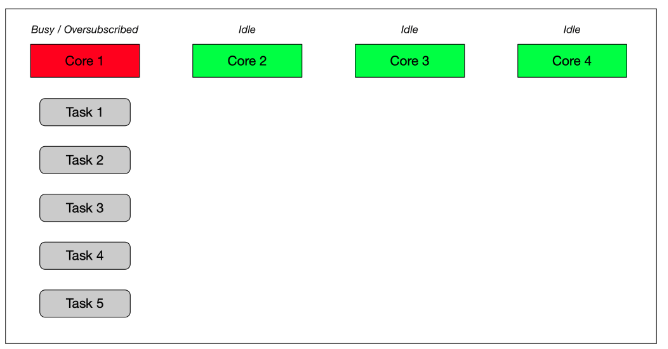
\includegraphics[width=.9\linewidth]{task_dist_1}  
  \caption{Before}
	\label{fig:before}
\end{subfigure}
\begin{subfigure}{.5\textwidth}
  \centering
  % include second image
  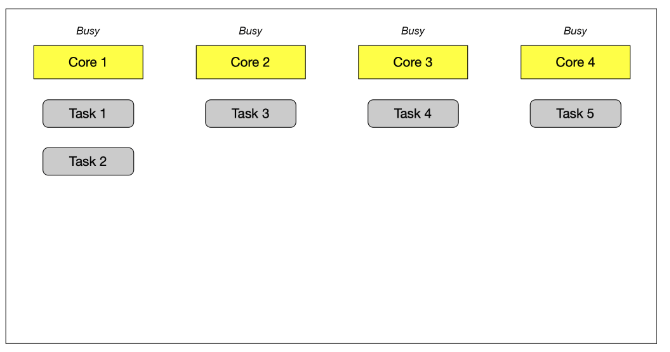
\includegraphics[width=.9\linewidth]{task_dist_2}  
  \caption{After}
	\label{fig:after}
\end{subfigure}
\caption{Work Stealing Queues}
\label{fig:work_stealing_queues}
\end{figure}





\textbf{Task-based vs Thread-based} programming:

\begin{table}[htpb!]
	\centering
	\caption{Tasks vs Threads}
	\label{tab:tasks_vs_threads}
	\begin{tabular}{|c|c|}
		\hline
	  \textbf{Task-based} & \textbf{Thread-based} \\
		\hline
		\hline
	  System takes care of many detail  & Programmer is responsible \\
		(e.g. join) &  for many details \\
		\hline
		Light-weight  & Heavy-weight (they are generated by the OS) \\
		because they will be using a & It takes time for the OS \\
		pool of already created & to allocate memory / stack /  \\
		threads  & kernel data for the thread \\
		\hline
		Cheaper to destroy    & Expensive to destroy \\
		\hline
		Focused on throughput & Focused on latency \\
	  \hline
		Concurrency abstraction is high & Concurrency abstraction is low \\
		\hline

	\end{tabular}
\end{table}



Threads have more to do with latency. When you have functions that can block (e.g. file input, server connection), threads can avoid the program to be blocked, when e.g. the server is waiting for a response. Tasks on the other hand focus on throughput, where many operations are executed in parallel.


In the file \texttt{performanceOfThreads.cpp} the main idea is to see if executing the threads in parallel makes sense. The parameters that we can change are \texttt{nLoops, nThreads, std::launch::async or deferred}. The result is that is we have a small number of loops, it doesn't make sense to run them in parallel. 



\subsubsection{Outro}%
\label{ssub:outro}

So we have two basic possibilities to start threads. We can either use \texttt{std::thread}  or \texttt{std::async}. As a general rule of thumb, using async as in many cases is the easiest solution which involves less boilerplate code and basically you can achieve the same as with \texttt{std::thread}. With async you don't have to worry about calling \texttt{join()}  in the parent thread and also there's no \textbf{promise} you need to carry around and manage. 

We might consider using threads when we want to have more control. Don't think to use async to launch tasks that do input-output manipulate mutexes or in other ways, interact with other threads. The idea is to use async in the simples and more common cases. 



\subsection{Avoiding Data Races}%
\label{sub:avoiding_data_races}

\textbf{Data Races} occur, when two concurrent threads are accessing the same memory location while at least one of them is modifying (the other thread might be reading or modifying). In this scenario, the value at the memory location is completely undefined. Depending on the system scheduler, the second thread will be executed at an unknown point in time and thus see different data at the memory location with each execution. Depending on the type of program, the result might be anything from a crash to a security breach when data is read by a thread that was not meant to be read, such as a user password or other sensitive information. Such an error is called a data race because two threads are racing to get access to a memory location first, with the content at the memory location depending on the result of the race.




We'll discuss some strategies for avoid them:

\begin{enumerate}
	\item Overwriting the copy constructor of a class to ensure a proper deep copy of all data structures as performed.  
	\item Move semantics 
	\item carefully synchronize the two threads using the \texttt{join()} or the promise-future concept that can guarantee the availability of a result.
\end{enumerate}



In the file \texttt{DataRaceExample\_atomic.cpp}, an instance of the proprietary class \texttt{Vehicle} is created and passed to a thread by value, thus making a copy of it.

Note that the class Vehicle has a default constructor and an initializing constructor. In the main function, when the instances v0 and v1 are created, each constructor is called respectively. Note that v0 is passed by value to a Lambda, which serves as the thread function for std::async. Within the Lambda, the id of the Vehicle object is changed from the default (which is 0) to a new value 2. Note that the thread execution is paused for 500 milliseconds to guarantee that the change is performed well after the main thread has proceeded with its execution.

In the main thread, immediately after starting up the worker thread, the id of v0 is changed to 3. Then, after waiting for the completion of the thread, the vehicle id is printed to the console.


\textit{Note: We can't get the value of v0 to be equal to 2 because it's passed by value. If it were passed by reference, we can print out the value in the main thread. This is in file DataRaceExample\_atomic.cpp}




Passing data to a thread in this way is a clean and safe method as there is no danger of a data race - at least when atomic data types such as integers, doubles, chars or booleans are passed.


Now, in the file \texttt{DataRaceExample\_pointer.cpp} we show the fact that when passing a complex data structure however, there are sometimes pointer variables hidden within, that point to a potentially shared data buffer - which might cause a data race. 


Even though v0 is being copied by value when passed to the thread function, this time, however, even though a copy has been made, the original object \texttt{v0} is modified, when the thread function sets the new name. This happens because the member \texttt{\_name} is a pointer to a string and after copying, even though the pointer variable has been duplicated, it still points to the same location as its value (i.e. the memory location) has not changed. Note that when the delay is removed in the thread function, the console output varies between "Vehicle 2" and "Vehicle 3", depending on the system scheduler. Such an error might go unnoticed for a long time. It could show itself well after a program has been shipped to the client





Classes from the standard template library usually implement a deep copy behavior by default (such as std::vector). When dealing with proprietary data types, this is not guaranteed. The only safe way to tell whether a data structure can be safely passed is by looking at its implementation: Does it contain only atomic data types or are there pointers somewhere? If this is the case, does the data structure implement the copy constructor (and the assignment operator) correctly? Also, if the data structure under scrutiny contains sub-objects, their respective implementation has to be analyzed as well to ensure that deep copies are made everywhere.



\textbf{Overwriting Copy Constructor}

The problem with passing a proprietary class is that the standard copy constructor makes a 1:1 copy of all data members, \textbf{including pointers to objects}. We would like a \textit{"Deep Copy"}, that is, copying the data to which the pointer refers. 


In the file \texttt{OverwriteCopyConstructor.cpp} we make a deep copy so that the program always prints "Vehicle 3" to the console, regardless of the delay within the thread function.

\textit{Note: In fact, in the DataRaceExample\_pointer.cpp example my program always output the value Vehicle 2 to the console.}



\subsubsection{Passing data using move semantics}%
\label{ssub:passing_data_using_move_semantics}

Even though a customized copy constructor can help us to avoid data races, it is also time (and memory) consuming. In the following, we will use move semantics to implement a more effective way of safely passing data to a thread.

A move constructor enables the resources owned by an rvalue object to be moved into an lvalue without physically copying it. Rvalue references support the implementation of move semantics, which enables the programmer to write code that transfers resources (such as dynamically allocated memory) from one object to another.

Unlike the default copy constructor however, the compiler does not provide a default move constructor. 


\subsubsection{Move Semantics and Uniqueness}%
\label{ssub:move_semantics_and_uniqueness}

As with the above-mentioned copy constructor, passing by value is usually safe - provided that a deep copy is made of all the data structures within the object that is to be passed. With move semantics , we can additionally use the notion of uniqueness to prevent data races by default. In the file \texttt{moveSemanticsAndUniqueness.cpp}  example, a \texttt{unique\_pointer} instead of a raw pointer is used for the string member in the Vehicle class.


\textbf{In this file, the move constructor transfers the unique pointer to the worker by using \texttt{std::move}  and thus invalidates the pointer in the main thread.} When calling \texttt{v0.getName()}, an exception is thrown, making it clear to the programmer that accessing the data at this point is not permissible - which is the whole point of using a unique pointer here as a data race will now be effectively prevented. 

The point of this example has been to illustrate that move semantics on its own is not enough to avoid data races. The key to thread safety is to use move semantics in conjunction with uniqueness. It's the responsibility of the programmer to ensure that pointers to objects that are moved between threads are unique.



\subsubsection{Outro}%
\label{ssub:outro}

A useful tip is to delay threads using standard sleep can help expose data races. And, one of the key things to thread safety is using move semantics in conjunction with uniqueness. It's the responsibility of the programmer to ensure that the pointers to objects that are moved between threads are always unique. 

Also, we can overwrite the copy constructor to enable a deep copy of a proprietary data structure or class. 



\section{Mutexes and Locks}%
\label{sec:mutexes_and_locks}


\subsection{Using a Mutex to Protect Sharing Data}%
\label{sub:using_a_mutex_to_protect_sharing_data}

The promise-future pair is for one time use only and only works in a single direction. With \texttt{mutex} we can safely \textbf{lock} a resource, modify it, and then unlock it again once we're done with it. 


\subsubsection{Using Mutex to Protect Shared Data}%
\label{ssub:using_mutex_to_protect_shared_data}


\textbf{The mutex Entity}

Until now, the methods we have used to pass data between threads were short-term and involved passing an argument (the promise) from a parent thread to a worker thread and then passing a result back to the parent thread (via the future) once it has become available. The promise-future construct is a non-permanent communication channel for one-time usage.

In C++, the concept of taking turns can be constructed by an entity called a \textbf{"mutex"} - which stand for Mutual Exclusion.


Recall that a data race requires simultaneous access from two threads. If we can guarantee that only a single thread at a time can access a particular memory location, data races would not occur. In order for this to work, we would need to establish a communication protocol. It is important to note that a \textbf{mutex} is not the solution to the data race problem per se but merely an enabler for a thread-safe communication protocol that has to be implemented and adhered to by the programmer.



\begin{figure}[htpb!]
	\centering
	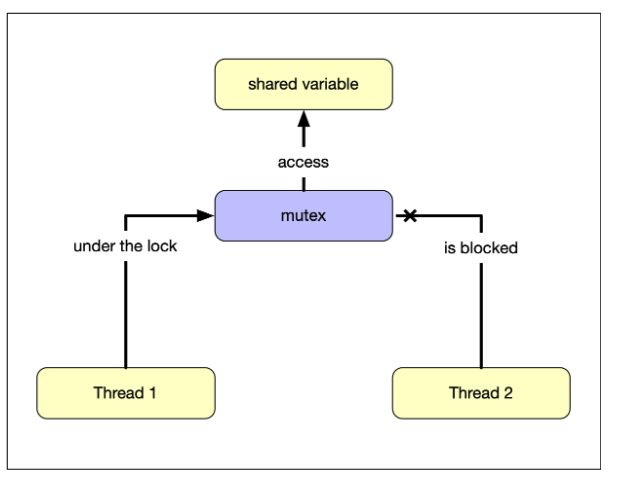
\includegraphics[width=0.8\linewidth]{mutex}
	\caption{Mutex}
	\label{fig:mutex}
\end{figure}




Let us take a look at how this protocol works: Assuming we have a piece of memory (e.g. a shared variable) that we want to protect from simultaneous access, we can assign a mutex to be the guardian of this particular memory. It is important to understand that a mutex is bound to the memory it protects. A thread 1 who wants to access the protected memory must "lock" the mutex first. After thread 1 is "under the lock", a thread 2 is blocked from access to the shared variable, it can not acquire the lock on the mutex and is temporarily suspended by the system.

Once the reading or writing operation of thread 1 is complete, it must "unlock" the mutex so that thread 2 can access the memory location. Often, the code which is executed "under the lock" is referred to as a "critical section". It is important to note that also read-only access to the shared memory has to lock the mutex to prevent a data race - which would happen when another thread, who might be under the lock at that time, were to modify the data.

When several threads were to try to acquire and lock the mutex, only one of them would be successful. All other threads would automatically be put on hold - just as cars waiting at an intersection for a green light. Once the thread who has succeeded in acquiring the lock had finished its job and unlocked the mutex, a queued thread waiting for access would be woken up and allowed to lock the mutex to proceed with his read / write operation. If all threads were to follow this protocol, a data race would effectively be avoided.

A complete example could be find in forcedDataRace.cpp. In the file, we commented out the \texttt{push\_back()} function. The reason is that we are trying to force a data race and if we keep \texttt{push\_back()} it'll cause the program to crash. Also, the tmp variable is used to see the data race. 


It seems that not all the vehicles could be added to the queue. But why is that? Note that in the thread function "pushBack" there is a call to sleep\_for, which pauses the thread execution for a short time. This is the position where the data race occurs: First, the current value of \_tmpVehicles is stored in a temporary variable oldNum. While the thread is paused, there might (and will) be changes to \_tmpVehicles performed by other threads. When the execution resumes, the former value of \_tmpVehicles is written back, thus invalidating the contribution of all the threads who had write access in the mean time. Interestingly, when sleep\_for is commented out, the output of the program is the same as with std::launch::deferred - at least that will be the case for most of the time when we run the program. But once in a while, there might be a scheduling constellation which causes the bug to expose itself. 

\textit{As an advice, introducing deliberate time delays in the testing / debugging phase of development can help expose many concurrency bugs.}


In its simples form, using a mutex consists of four straightforward steps:
\begin{enumerate}
\item include the $< mutex >$ header.
	\item Create and std::mutex
	\item Lock the mutex using lock() before read/write is called
	\item Unlock the mutex after the read/write operation is finished using unlock()
\end{enumerate}



In the file \texttt{mutex\_1.cpp} In order to protect the access to \_vehicles from being manipulated by several threads at once, a mutex has been added to the class as a private data member. In the pushBack function, the mutex is locked before a new element is added to the vector and unlocked after the operation is complete.

Note that the mutex is also locked in the function printSize just before printing the size of the vector. The reason for this lock is two-fold: First, we want to prevent a data race that would occur when a read-access to the vector and a simultaneous write access (even when under the lock) would occur. And second, we want to exclusively reserve the standard output to the console for printing the vector size without other threads printing to it at the same time.


Now, the data race will be avoided and the vector of vehicles will be 1000 always.


\subsubsection{Using Timed Mutex}%
\label{ssub:using_timed_mutex}

There different \texttt{mutex} types:

\begin{itemize}
	\item \texttt{mutex} provides the core functions \texttt{lock()} and \texttt{unlock()} and the non-blocking \texttt{try\_lock()} method that returns if the mutex is not available.
	\item \texttt{recursive\_mutex}: allows multiple acquisitions of the mutex from the same thread.
	\item \texttt{timed\_mutex} similar to mutex, but it comes with two more methods, \texttt{try\_lock\_for()} and \texttt{try\_lock\_until()} that try to acquire the mutex for a period of time or until a moment in time is reached. 
	\item \texttt{recursive\_timed\_mutex} combination of the previous two.
\end{itemize}

\begin{figure}[htpb!]
\begin{subfigure}{.5\textwidth}
  \centering
  % include first image
  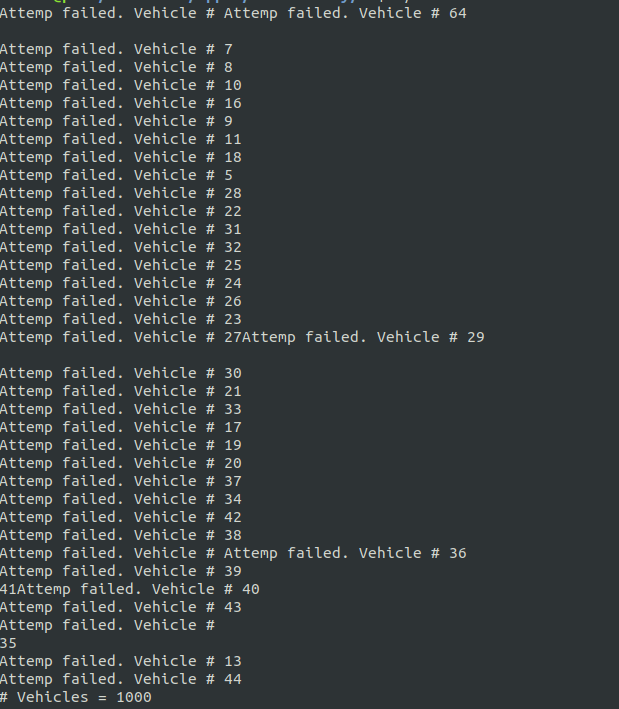
\includegraphics[width=.9\linewidth]{timed_mutex}  
  \caption{Timed Mutex i less than 3}
	\label{fig:timed_mutex}
\end{subfigure}
\begin{subfigure}{.5\textwidth}
  \centering
  % include second image
  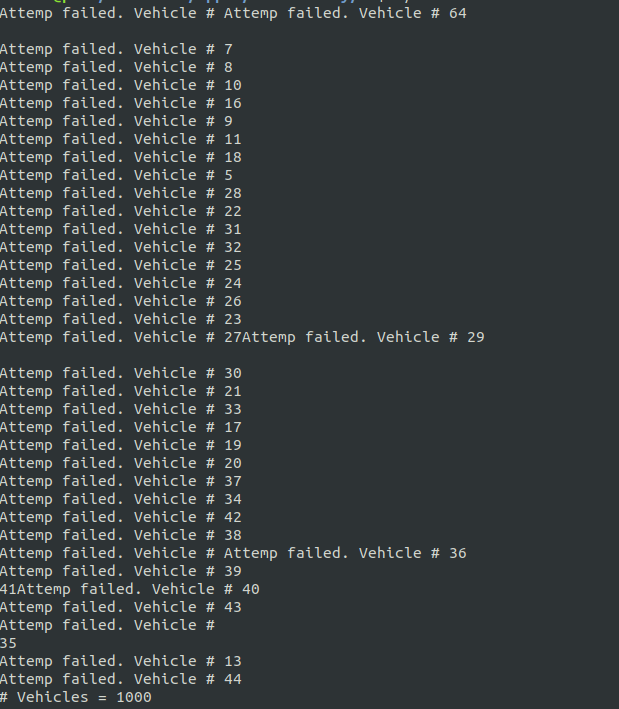
\includegraphics[width=.9\linewidth]{timed_mutex}  
  \caption{Timed Mutex i = 1}
	\label{fig:timed_mutex_1}
\end{subfigure}
\caption{Timed Mutex}
\label{fig:timed_mutex}
\end{figure}







\subsubsection{DeadLock}%
\label{ssub:deadlock}

Using mutexes can significantly reduce the risk of data races as seen in the example above. But imagine what would happen if an exception was thrown while executing code in the critical section, i.e. between lock and unlock. In such a case, the mutex would remain locked indefinitely and no other thread could unlock it - the program would most likely freeze.

In the file \texttt{deadlock\_1.cpp} we can see an output like Figure~\ref{fig:deadlock}.


\begin{figure}[htpb!]
	\centering
	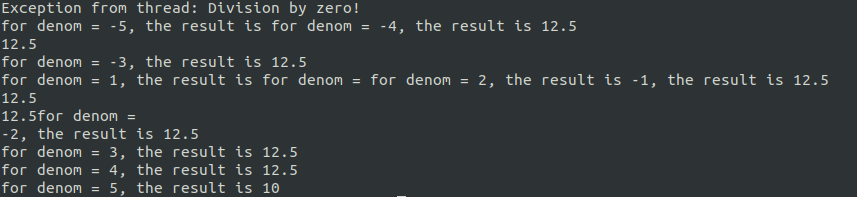
\includegraphics[width=0.8\linewidth]{deadlock}
	\caption{Deadlock}
	\label{fig:deadlock}
\end{figure}


So, what if we try to avoid this output by using mutexes? With the code added to the same file (codeadlock\_1.cpp), we get one type of deadlock, which causes a program to freeze because one thread does not release the lock on the mutex while all other threads are waiting for access indefinitely. 




A second type of \textbf{deadlock} is a state in which two or more threads are blocked because each thread waits for the resource of the other thread to be released before realising its resource. This is reflected in the file \texttt{deadlock\_2.cpp} 


\begin{figure}[htpb!]
	\centering
	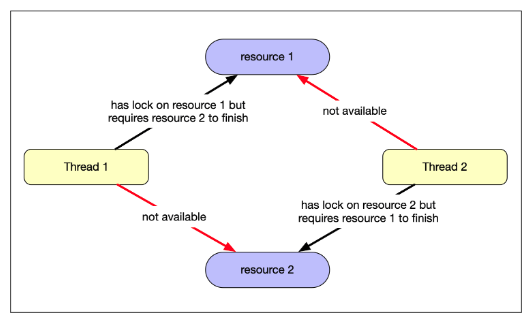
\includegraphics[width=0.8\linewidth]{deadlock_diagram}
	\caption{Deadlock Diagram}
	\label{fig:deadlock_diagram}
\end{figure}

In Figure~\ref{fig:deadlock_diagram} we see the logic of the deadlock.



\subsubsection{Using Locks to Avoid DeadLocks}%
\label{ssub:using_locks_to_avoid_deadlocks}


The basic idea is to package calls to the mutex in an object called a \texttt{lock\_guard} and this object lock's the mutex at the time of its creation and unlocks it automatically when it's destroyed. Now, imagine that in the middle of accessing a shared data location, there's an exception and the program flow is directed away from the current thread. As soon as the \texttt{lock\_guard} object is invalidated by going out of scope, the lock on the shared data is released and others can access it again. 

This concept can be extended further by a similar form called \texttt{unique\_lock}.


The idea of \textit{"working under the lock"} is to block access by other threads to the same resource. In practice, however, \textbf{direct calld to lock() shoudl be avoided at all cost!}. This can make us incur in the \textbf{deadlock problem} where while working under the lock, a thread would throw an expcetion and exit the critical section without calling the unlock function on the mutex. 

We can avoid this problem by creating a \texttt{std::lock\_guard} object, which keeps an associated mutex locked during the entire object life time. The lock is acquired on construction and released automatically on destruction. Also, \texttt{std::lock\_guard} guarantees exception safety because any critical section is automatically unlocked when an exception is thrown. 


This is in the file \texttt{lock\_guard.cpp}. 



\subsubsection{Unique Lock}%
\label{ssub:unique_lock}

The problem with the example in \texttt{lock\_guard.cpp} is that we can only lock the mutex once and the only way to control lock and unlock is by invalidating the scope of the \texttt{std::lock\_guard} object. 


A more flexible alternative to std::lock\_guard is uniquelock\_, that also provides support for more advanced mechanisms, such as deferred locking, time locking, recursive locking, transfer of lock ownership and use of condition variables (which we will discuss later). It behaves similar to lock\_guard but provides much more flexibility, especially with regard to the timing behavior of the locking mechanism.




In this version of the code, std::lock\_guard has been replaced with std::unique\_lock. As before, the lock object lck will unlock the mutex in its destructor, i.e. when the function divideByNumber returns and lck gets out of scope. In addition to this automatic unlocking, std::unique\_lock offers the additional flexibility to engage and disengage the lock \textbf{as needed by manually} calling the methods lock() and unlock(). This ability can greatly improve the performance of a concurrent program, especially when many threads are waiting for access to a locked resource. In the example, the lock is released before some non-critical work is performed (simulated by sleep\_for) and re-engaged before some other work is performed in the critical section and thus under the lock again at the end of the function. This is particularly useful for optimizing performance and responsiveness when a significant amount of time passes between two accesses to a critical resource.



The main advantages of unique\_lock over lock\_guard is that with unique\_lock you can:

\begin{itemize}
	\item construct an instance without an associated mutex using the default constructor
	\item construct an instance with an associated mutex while leaving the mutex unlocked at first using the deferred-locking constructor
	\item construct an instance that tries to lock a mutex, but leaves it unlocked if the lock failed using the try-lock constructor
	\item construct an instance that tries to acquire a lock for either a specified time period or until a specified point in time
\end{itemize}




Occasionally you can nest your locks, for example by calling a subsystem that protects its internal data with a mutex while holding a lock on another mutex, \textbf{but it is generally better to avoid locks on multiple mutexes at the same time, if possible.}
Sometimes, however, it is necessary to hold a lock on more than one mutex because you need to perform an operation on two different data elements, each protected by its own mutex.

We have seen that using several mutexes at once can lead to a deadlock, if the order of locking them is not carefully managed. To avoid this problem, \textbf{the system must be told that both mutexes should be locked at the same time}, so that one of the threads takes over both locks and blocking is avoided. That's what the std::lock() function is for - \textbf{you provide a set of lock\_guard or unique\_lock objects and the system ensures that they are all locked when the function returns.}  

An example of a deadlock with lock\_guard is in the file \texttt{lockguard\_deadlock.cpp}  and a way to avoid this is in \texttt{lockguard\_deadlockFree.cpp} we just add std::lock packing togheter 2 mutexes and add std::adopt\_lock to the std::lock\_guard.




\textit{As a rule of thumb, programmers should try to avoid using several mutexes at once. Practice shows that this can be achieved in the majority of cases. For the remaining cases though, using std::lock is a safe way to avoid a deadlock situation.}


\subsubsection{Outro}%
\label{ssub:outro}

Remember that mutexes should never be used directly even though this technically works. 

We can solve the dilemma of two locks depending of the unlocking of the other one with the standard lock operation (packing them together). 


\textbf{The 3 Lesson project}

The instance of class waiting vehicles is a \textbf{shared resource}: It's shared by all vehicles threads approaching intersection. And when one thread is \textbf{writing} and another thread is \textbf{either reading or writing} that's a \textbf{data race} regardless we observe an error or not at the time. 






\section{Condition Variables and Messages}%
\label{sec:condition_variables_and_messages}


The goal here is to develop a method for a controlled and finely range data exchange between several threads. In this lesson, we will build a concurrent message queue.

But, we first need to understand the \textbf{monitor object pattern and condition variables.}


\subsection{The Monitor Object Pattern}%
\label{sub:the_monitor_object_pattern}

This is a design pattern which is used to synchronize concurrent method execution to ensure that only one method at a time runs within an object. This is specially useful in cases where an application contains objects whose methods are invoked concurrently by multiple client threads and where these methods modify the state of their objects. 


What we would like to do now is to develop a mechanism that would allow us to react as soon as a new item was available. 



\textbf{Building the Monitor Object Pattern}

One important step towards such a construct is to implement a monitor object, which is a design pattern that synchronizes concurrent method execution to ensure that only one method at a time runs within an object. It also allows an object's methods to cooperatively schedule their execution sequences. The problem solved by this pattern is based on the observation that many applications contain objects whose methods are invoked concurrently by multiple client threads. These methods often modify the state of their objects, for example by adding data to an internal vector. For such concurrent programs to execute correctly, it is necessary to synchronize and schedule access to the objects very carefully. The idea of a monitor object is to synchronize the access to an object's methods so that only one method can execute at any one time.


In the file \texttt{printEntireVector.cpp}  we see that once the Vehicles are added to the WaitingVehicles vector, all are going to be printed out. 

While the pushBack method is used by the threads to add data to the monitor incrementally, the main thread uses printSize at the end to display all the results at once. Our goal is to change the code in a way that the main thread gets notified every time new data becomes available. But how can the main thread know whether new data has become available? The solution is to write a new method that regularly checks for the arrival of new data.



In the file \texttt{inifinitePollingLoop.cpp} we add a method \texttt{dataIsAvailable()}. This method return true if data is available in the vector and false otherwise. Once the main thread has found out that new data is in the vector, it can call the method \texttt{popBack()} to retrieve data from the monitor object. \textbf{Note that instead of copying the data, it is moved from the vector to the main method.}


\subsection{Building a Concurrent Message Queue}%
\label{sub:building_a_concurrent_message_queue}

The infinite polling loop puts a heavy load in the processor due to the constant iterations in very short intervals. One thing we could use is \textbf{futures} to fetch the data once we receive a signal that new data is coming. The problem with this is a that futures are meant to be used only once and for the purpose of our messaging queue we need a signaling mechanism that can be reused as often as we need it. This is where we use the \textbf{condition variable}


\subsubsection{Condition Variables}%
\label{ssub:condition_variables}

A std::condition\_variable has a method wait(), which blocks, when it is called by a thread. The condition variable is kept blocked until it is released by another thread. The release works via the method notify\_one() or the notify\_all method. The key difference between the two methods is that notify\_one will only wake up a single waiting thread while notify\_all will wake up all the waiting threads at once.

A condition variable is a low-level building block for more advanced communication protocols. It neither has a memory of its own nor does it remember notifications. Imagine that one thread calls wait() before another thread calls notify(), the condition variable works as expected and the first thread will wake up. Imagine the case however where the call order is reversed such that notify() is called before wait(), the notification will be lost and the thread will block indefinitely. So in more sophisticated communication protocols a condition variable should always be used in conjunction with another shared state that can be checked independently. Notifying a condition variable in this case would then only mean to proceed and check this other shared state.




\begin{figure}[htpb!]
\begin{subfigure}{.5\textwidth}
  \centering
  % include first image
  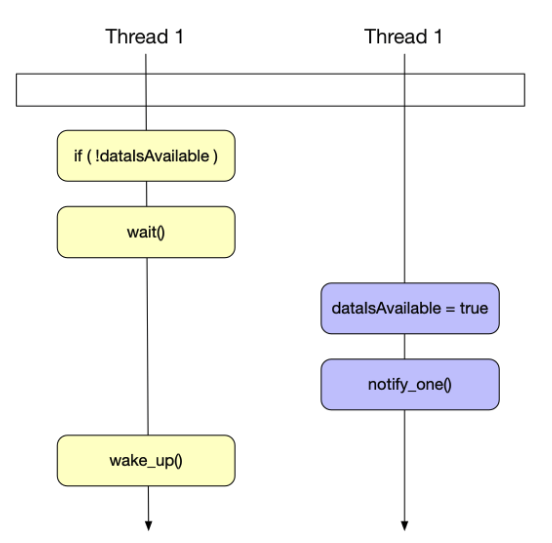
\includegraphics[width=.9\linewidth]{scenario_1}  
  \caption{Scenario 1}
	\label{fig:scenario_1}
\end{subfigure}
\begin{subfigure}{.5\textwidth}
  \centering
  % include second image
  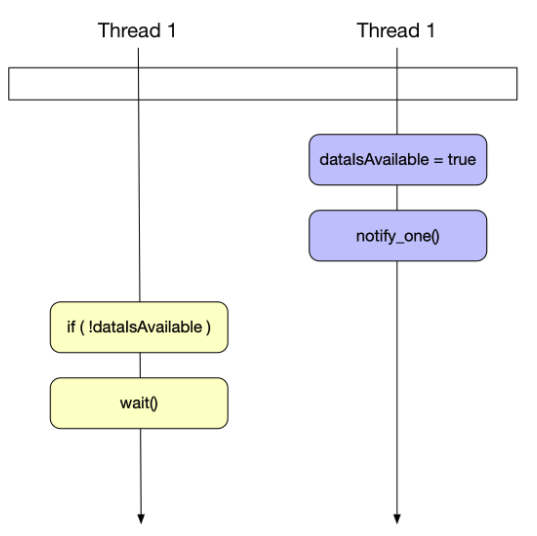
\includegraphics[width=.9\linewidth]{scenario_2}  
  \caption{Scenario 2}
	\label{fig:scenario_2}
\end{subfigure}
\caption{Communication Protocol}
\label{fig:communication_protocol}
\end{figure}




In the Scenario 1, the consumer thread checks dataIsAvailable() and since it is false, the consumer thread blocks and waits on the condition variable. Later in time, the producer thread sets dataIsAvailable to true and calls notify\_one on the condition variable. At this point, the consumer wakes up and proceeds with its work.

In the Sceneario 2, here, the producer thread comes first, sets dataIsAvailable() to true and calls notify\_one. Then, the consumer thread comes and checks dataIsAvailable() and finds it to be true - so it does not call wait and proceeds directly with its work. Even though the notification is lost, it does not cause a problem in this construct - the message has been passed successfully through dataIsAvailable and the wait-lock has been avoided.


In a non-concurrent environment, these two scenarios would most probably be sufficient to describe possible combinations. But, in a concurrent programming, because there are four atomic operators, two for each thread, when executed often enough, all possible interleaving will show themselves. 



In Figure~\ref{fig:lock_program} The consumer thread reads dataIsAvailable(), which is false in the example. Then, the producer sets dataIsAvailable() to true and calls notify. Due to this unlucky interleaving of actions, the consumer thread calls wait because it has seen dataIsAvailable() as false. The problem here is that after calling wait, the consumer thread will never wake up again. Also, as you may have noticed, the shared variable dataReady is not protected by a mutex here - which makes it even more likely that something will go wrong.


\begin{figure}[htpb!]
	\centering
	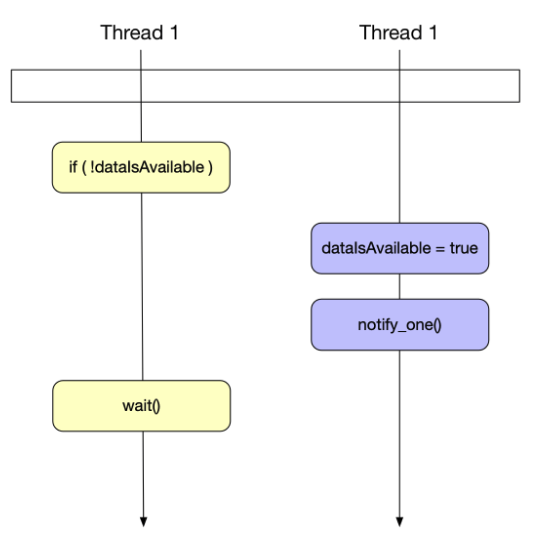
\includegraphics[width=0.8\linewidth]{lock_program}
	\caption{Lock Program}
	\label{fig:lock_program}
\end{figure}



One quick idea for a solution which might come to mind would be to perform the two operations dataIsAvailable and wait under a locked mutex. While this would effectively prevent the interleaving of tasks between different threads, it would also prevent another thread from ever modifying dataIsAvailable again.



This is shown in the Figure~\ref{fig:locked_mutex}. In there, we are closing the gap between reading the state and entering the wait. We are reading the state under the lock (red bar) and we call wait still under the lock. Then, we let wait release the lock and enter the wait state in one atomic step. This is only possible because the \textbf{wait()} method is able to take a lock as an argument. The lock that we can pass to wait however is not the lock\_guard we have been using so often until now but instead it has to be a lock that can be temporarily unlocked inside wait - a suitable lock for this purpose would be the unique\_lock type which we have discussed in the previous section.


\begin{figure}[htpb!]
	\centering
	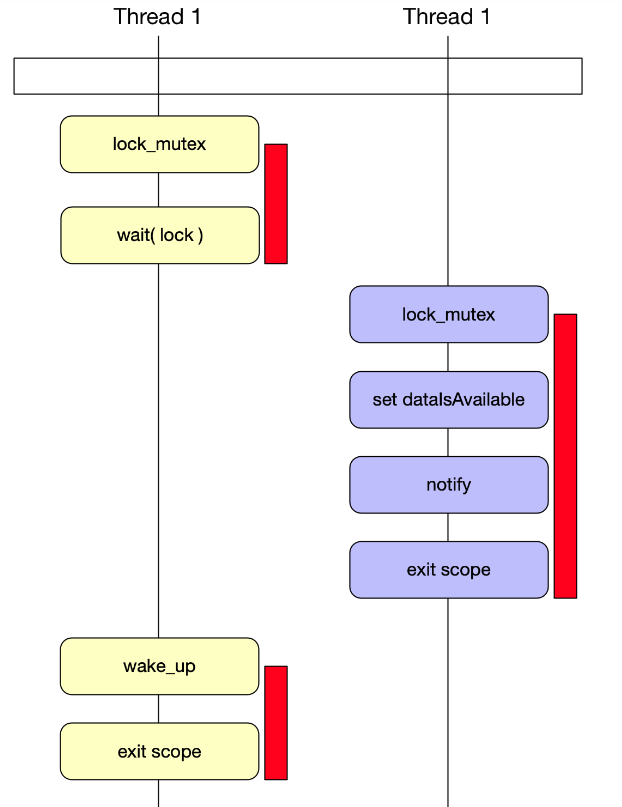
\includegraphics[width=0.8\linewidth]{locked_mutex}
	\caption{Locked Mutex}
	\label{fig:locked_mutex}
\end{figure}











\end{document}
